\documentclass[a4paper,12pt]{article}

% Packages for formatting
\usepackage{graphicx}  % For figures
\usepackage{amsmath, amssymb}  % For mathematical symbols
\usepackage{hyperref}  % For hyperlinks
\usepackage{booktabs}  % For tables
\usepackage{caption}  % For figure and table captions
\usepackage{geometry}  % Page layout
\usepackage{enumerate}
\usepackage{cite}
\usepackage{multirow}
\usepackage{booktabs}
\geometry{margin=1in}

\title{Data Analysis Report on House Prices Prediction using TFDF}
\author{Mohammad Hossein Basouli \\ Shahid Beheshti University of Tehran}
\date{\today}

\renewcommand{\thesection}{\Roman{section}} 
\renewcommand{\thesubsection}{\thesection.\Roman{subsection}}

\begin{document}

\maketitle

\begin{abstract}
    \textit{This report presents an analysis of a House Price Prediction work, done for a Kaggle competetion, in which we try to predict sale price of a house given many features. Also we would try to extract some of the most important features that have significant determinationation on the house sale price.}
\end{abstract}

\section{Data}
We have used the house \textbf{Ames Housing dataset} which was compiled by \textbf{Dean De Cock} \cite{ameshousingdataset2023}.
The data is represented as follows: each row is a record of a house (a total of 1460 training examples), along with 81 columns (80 features and the label \textbf{SalePrice}). The dataset includes both continous data and categorical data.
To get a feel of how the data look like, we present Figures 1 and Figure 2, representing how the label \textbf{SalePrice} and numerical features are being distributed respectively.

\begin{figure}[h] % 'h' means place the figure "here"
    \centering
    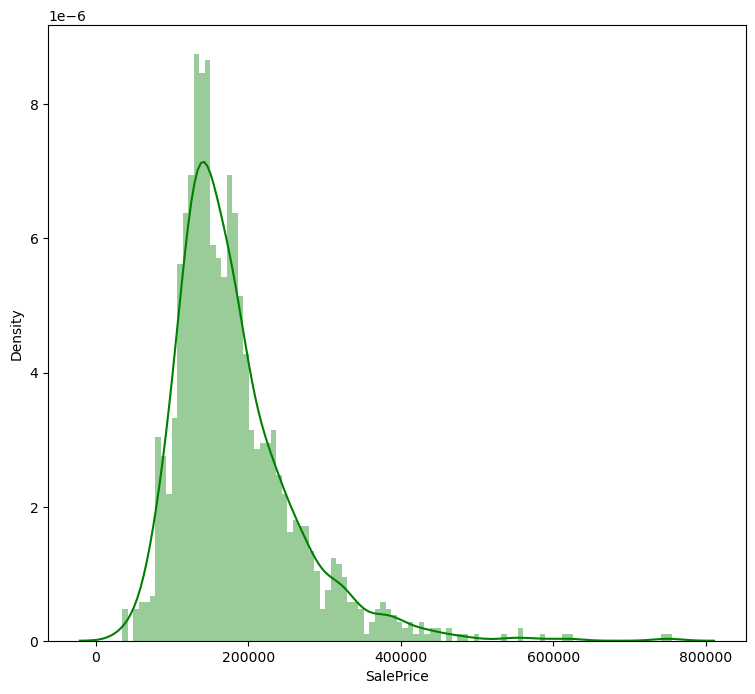
\includegraphics[width=0.5\textwidth]{./images/1.png} % adjust width and file path as needed
    \caption{Distribution of SalePrice}
\end{figure}

\begin{figure}[] % 'h' means place the figure "here"
    \centering
    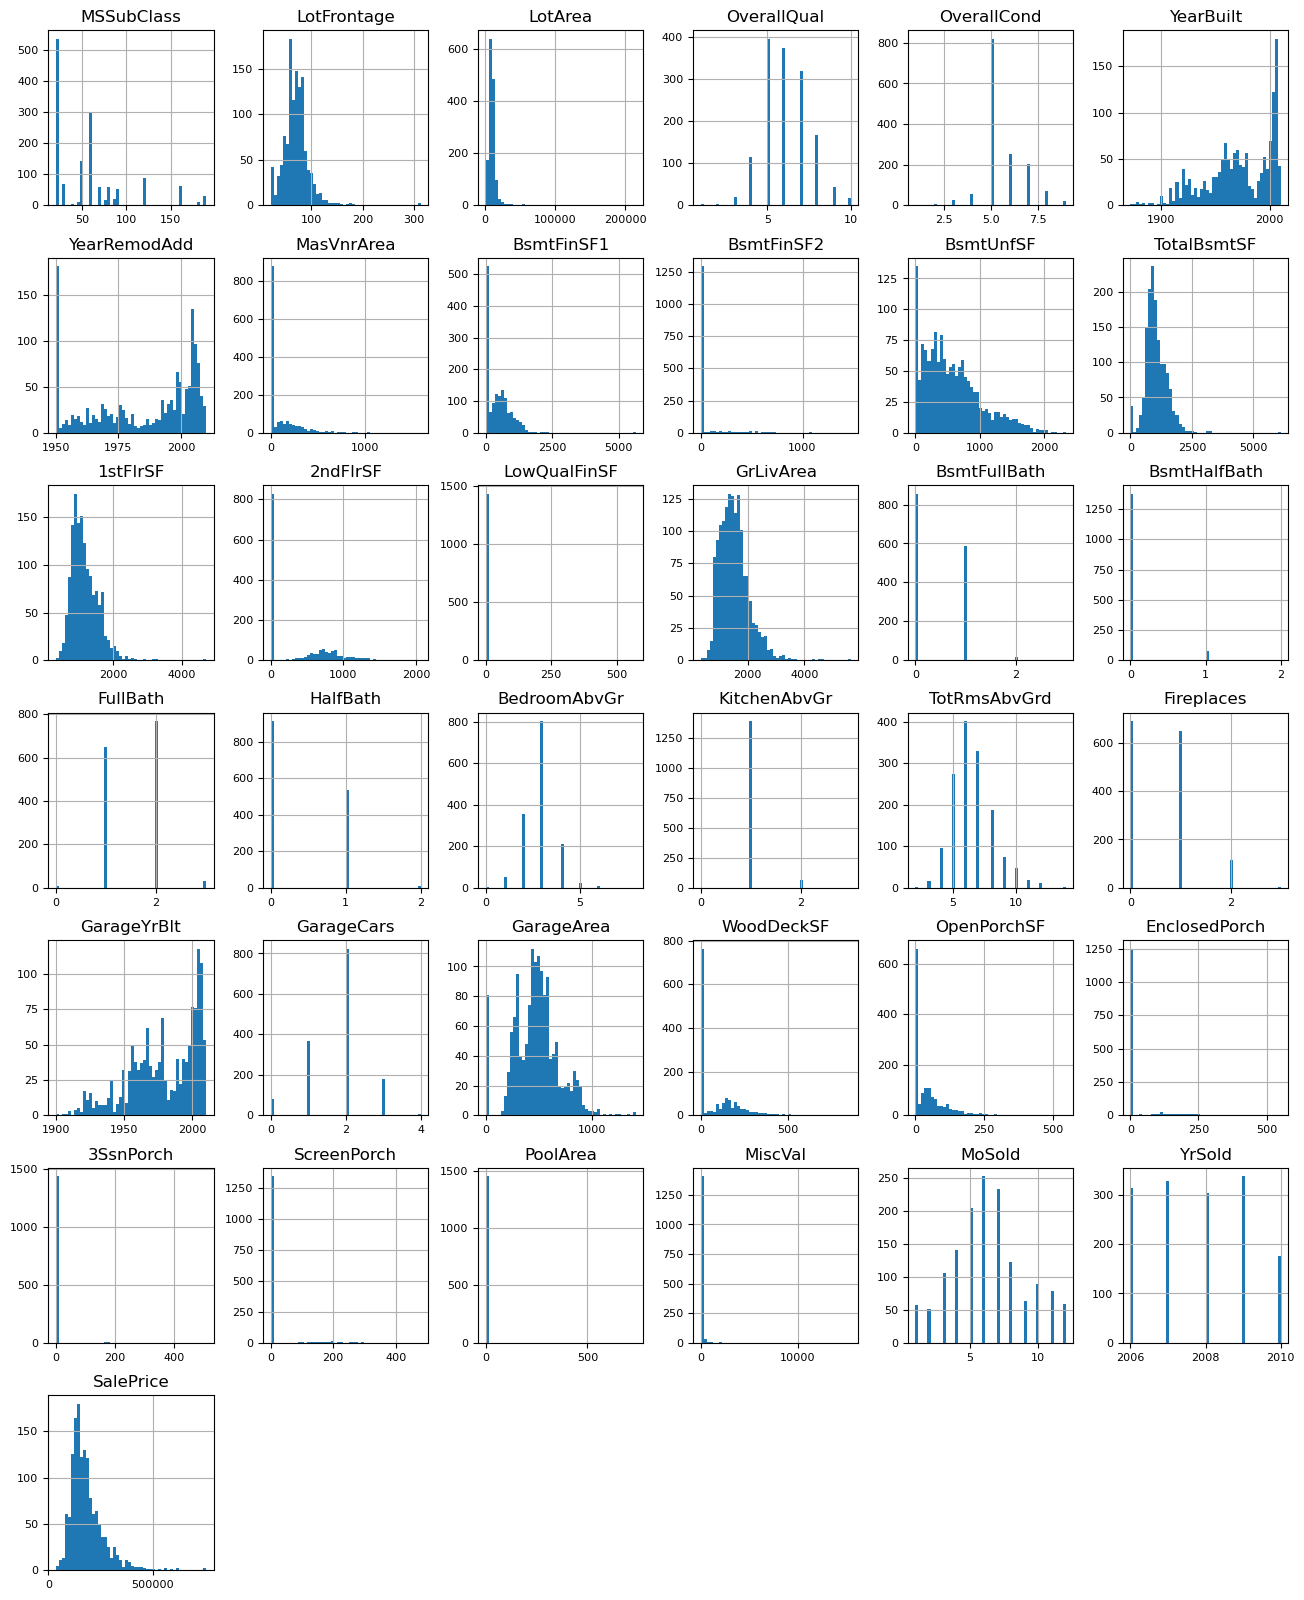
\includegraphics[width=0.5\textwidth]{./images/2.png} % adjust width and file path as needed
    \caption{Distribution of numerical features}
\end{figure}

\section{Features}
As mentioned earlier, the data includes both continous and categorical features. Some of the continous features are: lot area in squared feet, lot frontage, year sold and misc value. In addition, categorical features include street that the house is nearby to, alley that it's located in and shape of the lot.   

\section{Methodology: Random Forests}
\subsection{Strategy}
We have used Random Forests in order to learn insights from the data and predict the final \textbf{SalePrice} since, they work very well in situations where we have a mix of numeric, categorical and missing features and there is no need for any preprocessing.
Firstly we split the dataset into two pieces; train dataset and validation dataset, each having a size of 30\% and 70\% of the original dataset respectively and train our model.

\subsection{Result}
Our resutls of evaluation of the model can be seen in Figure 3 and Table 2 at the top of the following page as well as important features and their measure of importance based on number of times that they have been selected as the root in the trees in Figure 4 shown at the bottom of the following page.

\begin{figure}[] % 'h' means place the figure "here"
    \centering
    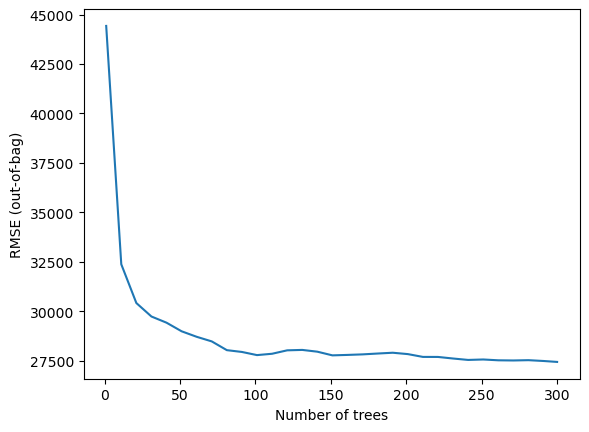
\includegraphics[width=0.5\textwidth]{./images/3.png} % adjust width and file path as needed
    \caption{Evaluation on the Out of bag (OOB) data}
\end{figure}

\begin{table}[htbp]
    \centering
    \caption{RMSE for Out-of-Bag (OOB) and Testing Data}
    \label{tab:classifiers}
    \begin{tabular}{lcc}
    \toprule
    & \textbf{OOB data RMSE} & \textbf{Testing data RMSE} \\
    \midrule
    Random Forests & 27438.6758 & 33064.0629 \\
    \bottomrule
    \multicolumn{3}{c}{\footnotesize Note: All results are based on dataset size of 470} \\
    \end{tabular}
\end{table}

\begin{figure}[] % 'h' means place the figure "here"
    \centering
    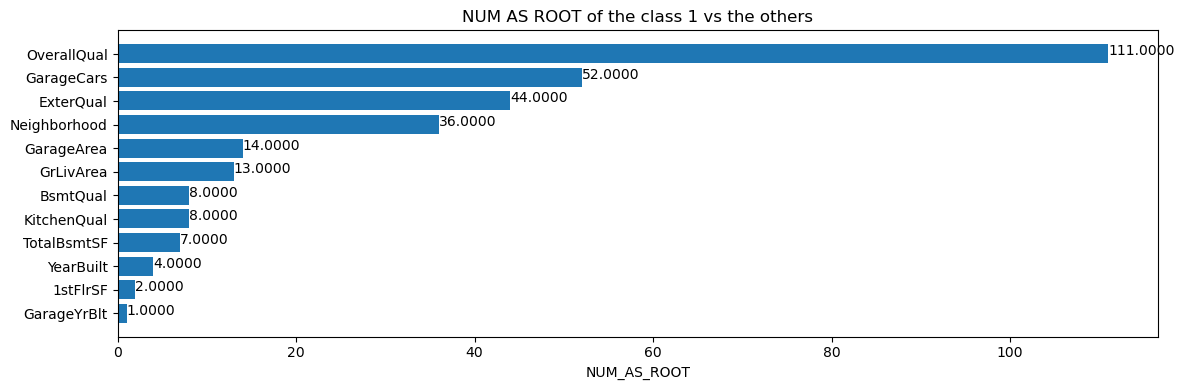
\includegraphics[width=0.5\textwidth]{./images/4.png} % adjust width and file path as needed
    \caption{Number of times as root for each of the important features}
\end{figure}


\subsection{Analysis}
Looking at Figure 1, we can see that our model makes a pretty good prediction based on observable statistics about \textbf{SalePrice}. Also, we can see that four of the features seem to be really important in the prediction of the \textbf{SalePrice}: \textbf{Overall Quality, Number of Cars that could be put in the Garage, Exteriror Quality of the house and Neighborhood}

\section{Conclusion}
We can conclude that core, well-known components of a house (such as those mentioned in the \textbf{Analysis} section) play a crucial role in determining the final \textbf{SalePrice} of the house.

% Bibliography Section
\bibliographystyle{ieeetr} % Choose a citation style (e.g., plain, apalike, ieeetr)
\bibliography{references} % Link to your .bib file

\end{document}
